\documentclass[onecolumn, draftclsnofoot,10pt, compsoc]{IEEEtran}
\usepackage{graphicx}
\usepackage{url}
\usepackage{setspace}

\usepackage{geometry}
\geometry{textheight=9.5in, textwidth=7in}
\title{CS462 Midterm Report}
% 1. Fill in these details
\def \CapstoneTeamName{		Team Phaze}
\def \CapstoneTeamNumber{		53}
\def \GroupMemberOne{			Alessandro Lim}
\def \GroupMemberTwo{			Jaydeep Rotithor}
\def \GroupMemberThree{			Touku Cha}
\def \CapstoneProjectName{		Evaporometer}
\def \CapstoneSponsorCompany{	Openly Published Environmental Sensing Lab}
\def \CapstoneSponsorPerson{		Chet Udell}

% 2. Uncomment the appropriate line below so that the document type works
\def \DocType{		%Problem Statement
				%Requirements Document
				%Technology Review
				%Design Document
				Progress Report
				}
			
\newcommand{\NameSigPair}[1]{\par
\makebox[2.75in][r]{#1} \hfil 	\makebox[3.25in]{\makebox[2.25in]{\hrulefill} \hfill		\makebox[.75in]{\hrulefill}}
\par\vspace{-12pt} \textit{\tiny\noindent
\makebox[2.75in]{} \hfil		\makebox[3.25in]{\makebox[2.25in][r]{Signature} \hfill	\makebox[.75in][r]{Date}}}}
% 3. If the document is not to be signed, uncomment the RENEWcommand below
%\renewcommand{\NameSigPair}[1]{#1}

%%%%%%%%%%%%%%%%%%%%%%%%%%%%%%%%%%%%%%%
\begin{document}
\begin{titlepage}
    \pagenumbering{gobble}
    \begin{singlespace}
    	
\includegraphics[height=4cm]{coe_v_spot1}
        \hfill 
        % 4. If you have a logo, use this includegraphics command to put it on the coversheet.
        %\includegraphics[height=4cm]{CompanyLogo}   
        \par\vspace{.2in}
        \centering
        \scshape{
            \huge CS Capstone \DocType \par
            {\large\today}\par
            \vspace{.5in}
            \textbf{\Huge\CapstoneProjectName}\par
            \vfill
            {\large Prepared for}\par
            \Huge \CapstoneSponsorCompany\par
            \vspace{5pt}
            {\Large\NameSigPair{\CapstoneSponsorPerson}\par}
            {\large Prepared by }\par
            Group\CapstoneTeamNumber\par
            % 5. comment out the line below this one if you do not wish to name your team
            \CapstoneTeamName\par 
            \vspace{5pt}
            {\Large
                \NameSigPair{\GroupMemberOne}\par
                \NameSigPair{\GroupMemberTwo}\par
                \NameSigPair{\GroupMemberThree}\par
            }
            \vspace{20pt}
        }
        \begin{abstract}
        % 6. Fill in your abstract    
        	This document is intended to be an overall status report on the Evaporometer project. Throughout this document, each group member states where they are on their section of the project, what they have left to do to complete their section, and what problems they faced. This document also contains additional relevant information for each section of the project along with diagrams to better illustrate progress. The first section of the document describes the status of the transmitter. The second section does so for the receiver. The third section gives a status update on the web mapping section of the project.
        \end{abstract}     
    \end{singlespace}
\end{titlepage}
\newpage
\pagenumbering{arabic}
\tableofcontents
% 7. uncomment this (if applicable). Consider adding a page break.
%\listoffigures
%\listoftables
\clearpage

% 8. now you write!
\section{Introduction}
The purpose of this project is to develop an open-source, automated data gathering systems that can be easily and inexpensively reproduced. The project is divided to 3 main parts: transmitter, receiver, and geovisualization. The transmitter gathers environmental data and sends the data to the receiver. The receiver receives the data and upload the data to a physical data storage and to the cloud database. The geovisualization portion takes the data and plots it into several different types of charts and a web map.


\section{Alessandro}
\subsection{Project Purposes and Goals}
The purpose of our project is to develop an automated data gathering system that can be easily used and reproduced. The project uses and Internet of Things system to send data between the data-gathering micro-controller unit and the receiving microcontroller unit. I am currently handling the data-gathering microcontroller unit (transmitter). The goal of the transmitter is to read temperature, humidity, albedo, and rainfall, and send the data to the receiver. 

\subsection{Current Standing}
I have been working closely with Touku on the communication between transmitter and the receiver. Currently, the transmitter can read temperature, humidity, lux intensity, and rainfall. The transmitter can also send those data into the receiver. However, the testing of the code has only been done on a breadboard instead of on the transmitter housing. The testing will be done as soon as the open-sensing team assemble the device on the transmitter housing.


First, I worked on the state diagram of the evaporometer transmitter code which was requested by the Open-sensing team. The goal of the state diagram is to visually explain the flow of the transmitter code so that the code is easily understandable.


Second, I worked on the wiring schematics and the documentation of the transmitter. The wiring schematics shows how to connect Adafruit Feather 32u4 to 1 DS3231 real time clock, 2 TSL2561 lux sensor, 1 SHT31-D humidity and temperature sensor, and 1 HX711 weighing sensor. The goal of the documentation is for easy replication and to show how the transmitter is assembled. The documentation listed the parts used by the transmitter and how to connect all those parts together.

\begin{figure}[ht]
\caption{The picture above is the schematic of the evaporometer transmitter. The schematic shows how all the evaporometer transmitter parts are connected together}
\centering
\includegraphics[width=17cm, height=15cm]{transmitter_bb.eps}
\end{figure}

Third, I worked on changing the light sensor code. The Open-sensing lab decided to use the TSL2561 light sensor instead of the TSL2591. The TSL2591 cannot be used to measure albedo since only one TSL2591 can be read by the microcontroller, and measuring albedo requires two lux sensors. The sensor handling library for both TSL2561 and TSL2591 is created by the parts supplier and is publicly available. Due to similarity of the TSL2561 and the TSL2591 handling library, the code structure is almost identical and porting the code was not a problem. 


Finally, another part that I worked on is looking up on how to send data from the receiver to mongoDB. I found out how to upload the data into the mongoDB without using the PushingBox API, and it can be applied to our project. However, the client has decided not to upload the data directly to mongoDB, and what I researched probably will not be applied to our project.
Currently, the transmitter code is ready for the live demo of the systems in the 5th of March. 

\subsection{Work Left}
First, the part that I’m going to work on next is assembling the device into the housing. The open-sensing team requested that I help them assemble the device. Assembling the device will be the first priority before the live demo on the 5th of march. I will work with them soon and I will test the transmitter code on the device once it has been assembled.


Second, the next part I’m going to work on is calibrating the weight sensor. Since the weight sensor is connected to a compartment that measures the rainfall, the initial weight is not going to be 0. I will have to calibrate the weight sensor so that it reads 0lbs when it is connected to the compartment. The calibration will also be one of the tasks required to finish before the 5h of March.


Third, the part that I’m going to work on is measuring albedo. While it is part of our main goal, the Open-sensing team has decided not to focus on measuring albedo for now. Measuring albedo simply requires two light sensors measuring light intensity, and the albedo is derived by dividing light intensity directly from the sun with the light intensity from the reflection of the sun. Measuring albedo and testing will be a focus after the live demo of the evaporometer. 


Fourth, another part that I’m going to work on is adding a button to the evaporometer that resets the evaporometer. If the button is pressed, the evaporometer will recalibrate the weight sensor of the rain-catcher system. While the code for the reset system has been done in a separate environment, it has not been added to the live system. It is not sure yet if the button will be in the final arrangement, but it will be decided after the live demo. 


Finally, the part that I’m going to work on is connecting an SD card reader on the transmitter. The SD card reader is to store the data gathered by the transmitter in case if the transmitter fails to send data to the receiver. It is also not sure if the SD card reader will be added to the final system of the evaporometer, but it will also be decided after the live demo.


\subsection{Impeded Problems}
In the first 3 to 4 weeks of the term, I did not make much progress on the project. I only did the part that the open-sensing team requested every week, which is mainly the state machine diagram and the documentation. I was also unsure on what I was supposed to be working on at the first few weeks. However, in the past two weeks, it has been clear what I am supposed to do, and the progress has been picking up quickly. 

\subsection{Other Information}
The Open-sensing team are still working on the final housing of the transmitter. The next transmitter housing is going to support albedo measuring and solar charging, which is not supported by the current housing. The final housing should be done after the live demo on the 5th of March is finished.


The Open-sensing team is going to show a live demo of the evaporometer project on the 5th of March. They are going to invite several professors to the lab and show the whole project to them. The alpha demo of the evaporometer project should be ready by then.
\section{Touku}
\subsection{Project Purposes and Goals}
The purpose of our project is to develop an open source, Internet of Things, weather station for researchers to gather data remotely.  Previously researchers traveled great distances to reach remote locations and gather data. With the Evaporometer researchers can to deploy weather stations and monitor them remotely without having to travel and grab the collected information.  The goals of our project are to develop up to 20 Evaporometers along with one central hub.

The Evaporometers will collect information such as rainfall, temperature, humidity,  and light (infrared, full spectrum, and albedo). The Evaporometers will collect data and transmit the data to the hub.  The hub will store and upload all the information to our database on Google Drive.  The hub will also use microSD as a backup storage device.

The priority is to upload the data straight to our Google Drive but use the SD card as a redundant storage in case network connectivity is lost.  A stretch goal we were given was to develop solar charging and Geo Visualization for the project.  Solar charging will ensure that the devices can operate 24/7 without needing battery changes.  The Geo Visualization will be used to map data points for researchers to use in future data comparisons.\\

\subsection{Current Standing}
Currently we are in the demo stage of our project.  The demo stage will include setting up the Evaporometer to transmit data and setting up the hub to collect and upload data.  My assignment is to get the hub up and running.  The hub will collect data from the Evaporometer and upload the data to our Google Spreadsheet via Pushing Box.  The hub is a Feather 32u4 attached with an Adafruit Featherwing with an Ethernet port. 

The Featherwing is hard wired into the network at HJ Andrews and the OPENs lab to have Internet connectivity.  I have finished setting up the PushingBox scenarios and services.  They are API function calls to our Google Spreadsheet.  PushingBox is connected to the Spreadsheet using the PushingBox API that allows us to call our Google Script.  The Google Script separates the data from PushingBox which comes as individual variables and inserts them into our spreadsheet.  The spreadsheet (currently) records: time stamp, ID tag (of the transmitter), temperature in Celsius, humidity, the load cell (for rainfall), infrared light, full spectrum light, battery voltage (of the transmitter), and the RSSI. 

The RSSI will be used to determine the radio strength of the transmission so we can find ideal locations to place them.  Documentation regarding the wiring diagrams and state machine diagrams have been sent to our team leads and client.  The wiring diagrams and state machine diagrams will be used by the OPENs team during their open house when they showcase the project.  The documentation serves as a quick and easy read for researchers to understand how our project works and how they can replicate the setup.\\

\subsection{Work Left: Data Upload}
The work I have left to do is to get the receiver to upload data correctly from the transmitter.  The receiver can receive the data transmission but is having issues separating the data correctly.  The transmitter sends the collected data as comma separated values which is then stored into an array.  From there the array is assigned to a value in PushingBox, such as \$IDTag\$, and pushed to the spreadsheet. 

\subsubsection{Issue and Solution}
My issue right now is that it is unable to convert the values correctly which is causing the receiver to send no data.  With no data it is unable to call the PushingBox function correctly leading to no data being transferred to our spreadsheet.  Along with that PushingBox nor the microcontroller will report that there is an issue.  It will only collect data and then transmit it, this process never returns an error message as the receiver believes its job is done.  The same for PushingBox, it will only notify us if a push to our spreadsheet was completed, no flag or error to notify us that something was trying to send but there was an issue. 

I believe the issue is with how the data is currently parsed from the transmitter to the array.  My solution is to re-implement the array in order to accommodate the values correctly.  From there I will do additional test on the PushingBox side to ensure that it is making the correct calls to our spreadsheet instead of doing nothing.\\

\subsection{Work Left: SD Storage}
\begin{figure}[ht]
\caption{A wiring diagram of the hub, the SD card is soldered onto the Feather while the Featherwing (Right) is stacked on top via headers}
\centering
\includegraphics[width=17cm, height=5cm]{receiver_evap1_bb.eps}
\end{figure}

The next thing that I am working on is the SD breakout board along with the SD card.  The SD breakout board is wired to the Feather 32u4 and programmed inside the microcontroller.  The issue I'm having with the breakout board is that the microcontroller is not detecting the SD breakout board and/or the SD card.  

\subsubsection{Issue and Solutions}
There are two issues and solutions that I think are causing the problem and will need to be addressed.  First I think the Feather 32u4 is not providing enough power to turn on the SD breakout board.  I believe this might be an issue with having the radio on the 32u4 turned on while the board is in use.  I will be testing the voltages of the board to determine if I need to turn off the radio while the breakout board is use.  If so, I can change the code to turn off the radio for the split second that data is being stored in the SD card.

The second issue may be related to how the SD card is formatted.  As of right now the card is formatted to FAT32.  However the technical document on Adafruit regarding this particular breakout board requires that the card be specially formatted into FAT32.  I will be loading up their software and formating the card accordingly to see if this will solve the issue.\\

\subsection{Other Information}
Once that is all figured out we will be meeting with our team leads at the OPENs lab to assemble the Evaporometer onto the PCB boards.  The PCB boards will be the resting place of our electronics where they will be installed inside a 3D printed model designed by our ECE team lead, Manuel.  The OPENs team will be hosting a open house of the project by March 5th.

This will allow us to practice before the engineering expo so we are aiming to get everything up before then.  Our goal is to have all the deliverables by February 21st or 28th depending on our client who has been injured. 

Other deliverables we have been working on is a bill of materials (BOM) for our client.  The BOM will contain all the parts required to build the Evaporometer plus hub.  A secondary BOM I provided was for the solar charging which has proved to be more expensive then our team leads have expected.  So we may or may not implement the solar charging depending on our client.  20 solar chargers will bring up the entire cost by up to \$1000 with each one costing roughly \~\$50 to build.

\section{Jaydeep}

\subsection{Project Purposes and Goals}
The main purpose of the geovisualization portion of the project is to visually organize the data collected by the Evaporometer devices from the H.J. Andrews research forest. This data would then be used to determine whether the Evaporometer devices could be deployed in other settings in future experiments.

\subsection{Current Standing}
I have created the web page for the map and the charts on which the data will be visualized. Currently, I have 2 different web pages, but I will most likely combine them into one in the future. I have also added a base map on which the data from the Evaporometer devices will be plotted. This base map was retrieved from mapbox.com, and I used the “outdoors” topographical map as my base map to give users more context about the location. I have also set up the general layout of the web pages, such that the map is at the top, the charts are below it, and there is a table at the bottom that will contain the past 5 days’ worth of data. I also have a socket.io connection working from the server to the client, and I can successfully send sample data through this connection. Finally, I have created several documents that detail the workflow of the project. These documents include: a system architecture state diagram, a sketch of the flow of data through the project, and sketches of the charts, map and table.

\subsection{Work Left}
 First, I need to finish setting up the charts on which the data will be modeled. In order to accomplish this, I will need to create the charts using the appropriate libraries. I will then need to plot the sample data onto the charts. I will need to make sure that the data is being appropriately plotted on different types of charts.
 
 
Currently, the data is being sent from the Evaporometer devices straight to Google Drive. However, our geovisualization project relies on MongoDB as a data source. As a result, we will need to create a converter that takes data from Google Drive and sends it to MongoDB. We also need to send the data from MongoDB through the server onto the webpage using the socket.io connection that has been created. From there, the data will be sent to the charts and web map in a format that can be read, so that the data can be modeled directly from there. 


I will also need to stratify the data based on type. For example, the system should allow the user to choose which dataset is being modeled, rather than throwing all of the data onto the maps and charts at once. To do this, I will need to create separate tabs for each data field so that the user can choose which dataset they want to see. Another way that I will stratify the data is based on time periods. For example, I will give users the option of selecting live data, daily averages or monthly averages.


The web map also needs to be set up to receive live data. Currently, I have added in a base map with topographic features. However, I will need to receive geographic coordinate data from the devices so that I can map the exact location of each measurement. If I know beforehand what the exact location of the devices is, I can populate the coordinate fields myself, but there is a possibility that the positions of the devices could be affected by weather, so this static location may not be completely accurate.

\subsection{Problems Faced}
The most significant roadblock that I have run into over the course of the project involves database selection. We want to use the MongoDB database to store data from the Evaporometer devices. The current plan regarding the web map is to pull data from MongoDB and read it into a server file. The data will then be transmitted to the client using socket.io. However, the data is currently being transmitted from the Evaporometer devices to a Google Spreadsheet. We could use this as our data source for the web map, but the issue with this would be that Google Spreadsheet has data limits, and as a result, some incoming data would be dropped. Our solution for this is to create a middle man software that moves data from the spreadsheet to MongoDB periodically. This would attempt to get around the data limits in spreadsheet, since MongoDB does not have these data limits. We have periodically gone back and forth on this with our clients, but we eventually resolved to continue using Google spreadsheets to log our data. The reason for this is that in order to log the data straight to MongoDB, the rest of the group would need to completely change the way their system works, and this would require a significant time investment on their part, whereas there already exists documentation on how to send data from Google Drive to MongoDB.


	A smaller roadblock that I ran into was configuring socket.io. I had never used socket.io previously, and as such, there was a steep learning curve for me. The biggest problem that I had with it was creating a connection from the server to the client. More specifically, I did not know how to use the “emit” functionality to send data from the server. However, after reading through several pieces of documentation, I was able to figure out the general workflow of socket.io and successfully sent all of the sample data to my client file. 

\subsection{Other Information}
In order to complete the project, I am working with Professor Bo Zhao. He is a professor in the college of Earth, Ocean and Atmospheric Sciences at Oregon State University. The web map and charts are all part of big data visualization, which involves taking large datasets and presenting them in a manner that is easy to understand. Since the flow of data from the devices is in real time, there will be a very large amount of data coming in, and if it is not properly collected and modeled, it will be very difficult to make sense of this data. This big data visualization is designed to collect many data samples over time, and as a result, the data could be compared at monthly or yearly intervals to give a better idea of climate change. Also, if the project is successfully deployed, more devices could be built and data could be collected from various other regions, such as deserts and coastal areas.



 Below I have included a diagram of the data flow for geovisualization:
\begin{figure}[ht]
\caption{The diagram below shows the flow of the data from the database through the web server out to the web client}
\centering
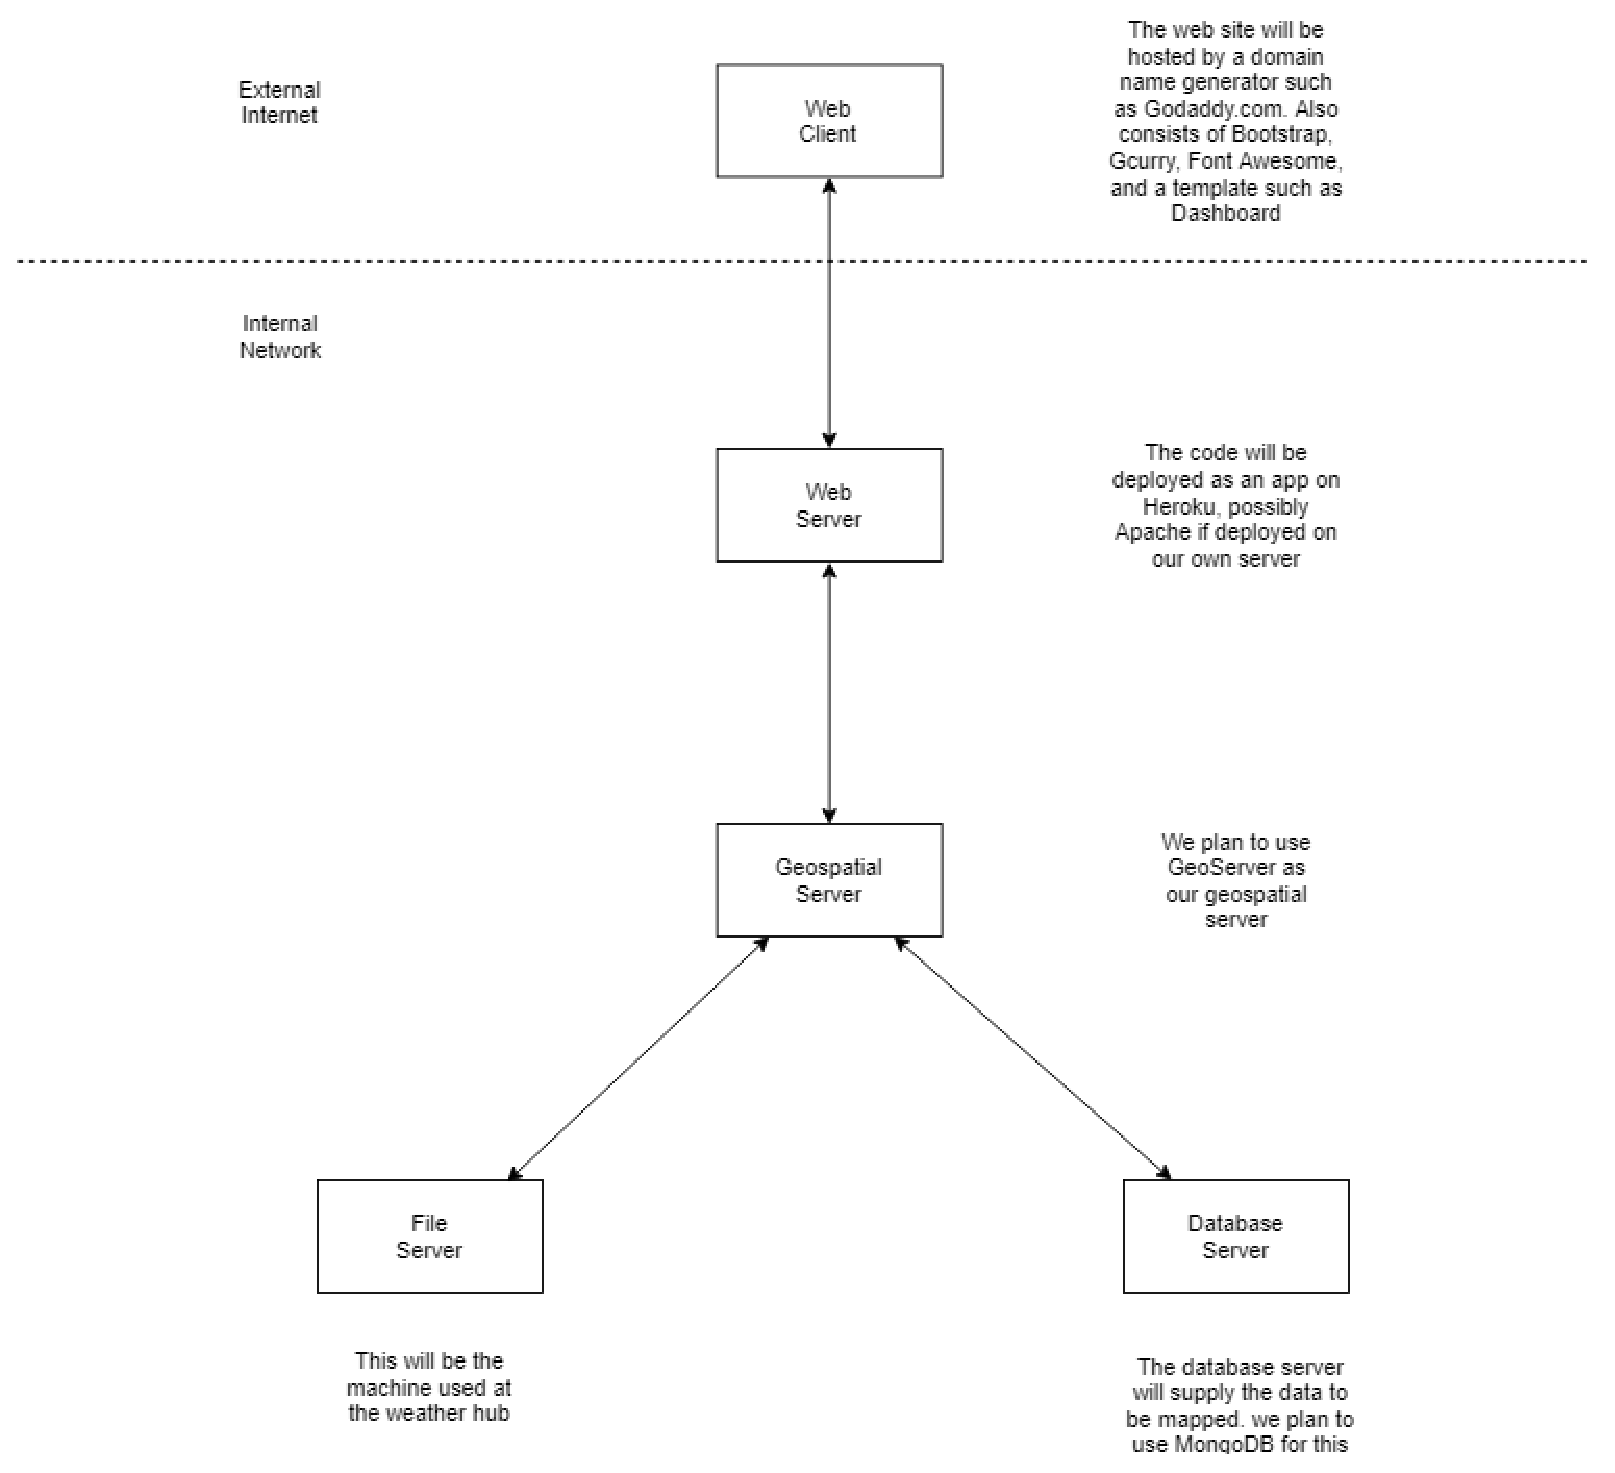
\includegraphics[width=10cm, height=9cm]{geoviz_flow.eps}
\end{figure}

\section{Conclusion}
	By March 5th we expect an Alpha build of our project to be ready for the open house.  The previous deadline for the open house was February 19th so we have extra time to include more functionality.  The transmitter once setup will be able to use all the sensors required for data collection.  For the receiver we will have it collect and upload data live during the open house.  We’re still working on collecting enough data so data visualization may or may not be up by the time we demo.

\end{document}